%\cleardoublepage %already included in mainmatter 
\chapter{Theoretical framework} \label{chapter2} %should be limited to 8 pages

% =====================================================================
\section{THM behaviors and spalling mechanisms} \label{sec:phenomena-spalling}

As heat rises within concrete, it undergoes a sequence of strongly interacting thermal, hydric, and mechanical processes. Heat causes the free and bound water inside the concrete to vaporize. Part of this vapour migrates inward and condenses in cooler regions, forming a quasi-saturated barrier known as a \emph{moisture clog}. This clog acts as an impermeable seal that prevents the remaining gas from escaping, which directly causes a severe pore-pressure build-up behind the drying front. Simultaneously, temperature gradients induce thermal stresses within the material. The full mathematical derivation of these THM behaviors is detailed in \cref{appendixA}.

These interacting phenomena are the root cause of \emph{spalling}. Explosive spalling generally results from the \emph{combined action} of pore pressure build-up and thermal stress (\cref{fig:spalling-mechanisms}).

\begin{figure}[htbp]
  \centering
  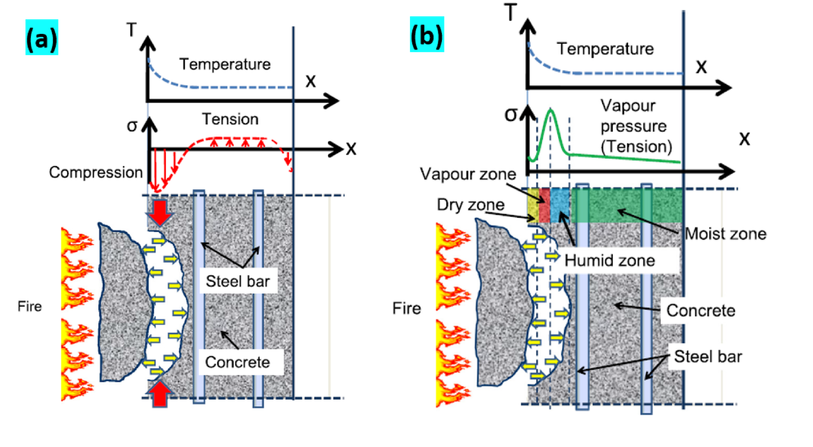
\includegraphics[width=0.7\linewidth]{figures/chapter2/spalling-mechanisms}
  \caption{Spalling combined mechanisms \cite{al-dalaien2025}}
  \label{fig:spalling-mechanisms}
\end{figure}

The spalling condition can be written schematically as:
\begin{equation}
    \sigma_{thermal}(T) + \sigma_{pore}(p_g,p_c,S_l) \ge f_t(T),
    \label{eq:spalling}
\end{equation}
where $\sigma_{thermal}$ is the thermal stress from differential dilation, $\sigma_{pore}$ the stress from pore-pressure loading, and $f_t(T)$ the temperature-degraded tensile strength. A comprehensive breakdown of this combined spalling mechanism is provided in \cref{sec:THM_spalling_app}.

\section{Improved thermo-hydro-chemical (THC) model} \label{sec:thcmodel}

\subsection{Motivation}
In standard Thermo-Hydric (TH) models, dehydration is treated through a fixed function of temperature alone - $\dot m_{dehyd}(T)$ and the porosity follows a simple linear law (as detailed in \cref{appendixA}). These simplifications overlook three facts that strongly affecting spalling:

\begin{enumerate}

\item The \emph{chemical state} of the cement paste before the accident depends on its hydration/curing history; 
\item The release of chemically bound water from the C--S--H is the chemical process that controls porosity, permeability and strength at high temperature; 
\item The chemical damage is essentially \emph{irreversible}. 

\end{enumerate} 
The improved Thermo-Hydro-Chemical (THC) model adopted here, following Scium\`e, Moreira and Dal~Pont \cite{sciume2024}, resolves the chemical field explicitly and couples it strictly to the thermal and hydric fields.

\subsection{Chemical state variables}
Unlike standard TH models, the THC framework explicitly resolves the chemical state of the cement paste. The evolution of the microstructure depends on two main processes \cite{sciume2024}:
\begin{itemize}
    \item \textbf{Hydration degree $\Gamma(t) \in [1]$:} Defines the formation of Calcium-Silicate-Hydrates (C-S-H) during curing and aging. Its evolution is governed by an Arrhenius-type chemo-kinetic law (detailed in \cref{sec:affinity}), driven by time, temperature, and relative humidity.
    \item \textbf{Dehydration degree $F(T) \in [1]$:} Represents the irreversible release of chemically bound water at high temperatures (typically $T > 105^\circ\mathrm{C}$).
\end{itemize}
To couple these effects, the \textbf{effective hydration degree} $\tilde{\Gamma}$ is introduced as the primary internal variable describing the state of the solid matrix:
\begin{equation}
    \tilde{\Gamma} = (1 - F(T))\,\Gamma
    \label{eq:effective-hydration}
\end{equation}
The transport and mechanical properties, such as porosity $\phi(\tilde{\Gamma})$ and intrinsic permeability $K(\tilde{\Gamma})$, are explicitly updated as functions of this effective hydration state. The specific evolution laws for these microstructural properties are detailed in \cref{sec:chemical_microstructure}.

\subsection{Resulting coupled system}
The standard Thermo-Hydric (TH) conservation equations for dry air, water species, and energy are detailed in \cref{eq:dry_air,eq:water_species,eq:energy_TH} of \cref{appendixA}. In these conventional formulations, the microstructural and chemical changes (e.g., the dehydration mass source $\dot{m}_{dehyd}$ and the porosity evolution) are treated implicitly via empirical functions of temperature alone.

By incorporating Powers' stoichiometry and the chemical couplings through the effective hydration degree $\tilde{\Gamma}$, the original system is profoundly transformed. The empirical functions are completely replaced by explicit chemo-physical interactions, reducing the final system to three highly non-linear conservation equations for the state variables $(p_g, p_c, T)$:

\paragraph{1. Dry-air conservation:}
\begin{equation}
    \underbrace{\frac{\partial}{\partial t}\big(\phi(1-S_l)\rho_a\big)}_{\text{Storage}} + \underbrace{\nabla \cdot (\mathbf{J}_a)}_{\text{Advection \& Diffusion}} = \underbrace{(1 - S_l)\rho_a \left(a_\phi \Omega \frac{\partial \tilde{\Gamma}}{\partial t}\right)}_{\text{Chemical coupling (porosity evolution)}}
\end{equation}

\paragraph{2. Total water-species conservation:}
\begin{equation}
    \underbrace{\frac{\partial}{\partial t}\big(\phi S_l \rho_l + \phi(1-S_l)\rho_v\big)}_{\text{Storage (Liquid + Vapor)}} + \underbrace{\nabla \cdot (\mathbf{J}_l + \mathbf{J}_v)}_{\text{Advection \& Diffusion}} = \underbrace{\left[ S_l\rho_l + (1-S_l)\rho_v \right] \left( a_\phi \Omega \frac{\partial \tilde{\Gamma}}{\partial t} \right)}_{\text{Porosity evolution}} - \underbrace{0.228 c \xi_\infty \frac{\partial \tilde{\Gamma}}{\partial t}}_{\text{De/hydration water source}}
\end{equation}

\paragraph{3. Energy conservation:}
\begin{equation}
    \underbrace{\overline{\rho C_p}\frac{\partial T}{\partial t}}_{\text{Heat storage}} + \underbrace{\mathbf{J}_{energy}^{adv}}_{\text{Advective heat flux}} - \underbrace{\nabla \cdot (\lambda \nabla T)}_{\text{Conduction}} = \underbrace{-H_{vap}\dot{m}_{vap}}_{\text{Phase change (Evaporation)}} + \underbrace{\left(H_{vap} 0.228 c \xi_\infty + L_{hyd}\right) \frac{\partial \tilde{\Gamma}}{\partial t}}_{\text{De/hydration latent heat}}
\end{equation}
where $a_\phi$ is the porosity evolution parameter, $c$ is the cement content, and $\xi_\infty$ is the maximum hydration fraction. The explicit formulation of these stoichiometric constants (e.g., the bound water $0.228 c \xi_\infty$ and the latent heat $L_{hyd}$) as well as the thermal activation energy $E_a/R$ governing $\tilde{\Gamma}$ are detailed in \cref{sec:powers} and \cref{sec:affinity} of \cref{appendixA}.

\section{Coupling to the mechanical field} \label{sec:mech}
The mechanical response is driven by the converged TH/THC fields through a \emph{one-way} (staggered) coupling: at each time step, the fields $(T,p_g,p_c)$ enter the mechanical problem as prescribed loading, and the resulting damage $\mathcal{D}$ feeds back weakly to the transport properties via permeability evolution at the next step. The TH/THC fields act through two routes:
\begin{itemize}
    \item \textbf{Free strains.} The total strain is decomposed as $\boldsymbol{\varepsilon}=\boldsymbol{\varepsilon}_\sigma+\boldsymbol{\varepsilon}_{th}+\boldsymbol{\varepsilon}_{sh}$, where $\boldsymbol{\varepsilon}_{th}$ is the thermal dilation (driven by $T$) and $\boldsymbol{\varepsilon}_{sh}$ the capillary shrinkage (driven by $p_c$). Creep is neglected, so $\boldsymbol{\varepsilon}_\sigma=\boldsymbol{\varepsilon}_{el}$.
    \item \textbf{Pore-pressure loading.} Through Bishop's effective stress $\boldsymbol{\sigma}'=\boldsymbol{\sigma}^{Total}+\alpha\,p_s\,\mathbf{I}$, the average pore pressure $p_s=p_g-S_l p_c$ enters the load vector as an external loading; its build-up shifts $\boldsymbol{\sigma}'$ towards tension and promotes cracking when $f_t(T)$ is exceeded.
\end{itemize}
Together with the spalling criterion \eqref{eq:spalling}, this closes the physical loop between the transport and mechanical fields. The mechanical constitutive model, its fracture-energy regularisation, and the spatial/temporal discretisation of the coupled problem are reported in full in \cref{appendixA}. 

\textbf{Note on the scope of the study:} Due to the limited timeframe of the internship and the fact that the experimental data used for validation (Kalifa test) solely provide temperature and gas pressure measurements, the mechanical module cannot be rigorously validated. Therefore, while this staggered mechanical coupling is mathematically formulated and designed as an easily pluggable module, the actual numerical simulations performed in the subsequent chapters are restricted to the TH(C) model.
